


\tikzset{every picture/.style={line width=0.75pt}} %set default line width to 0.75pt        

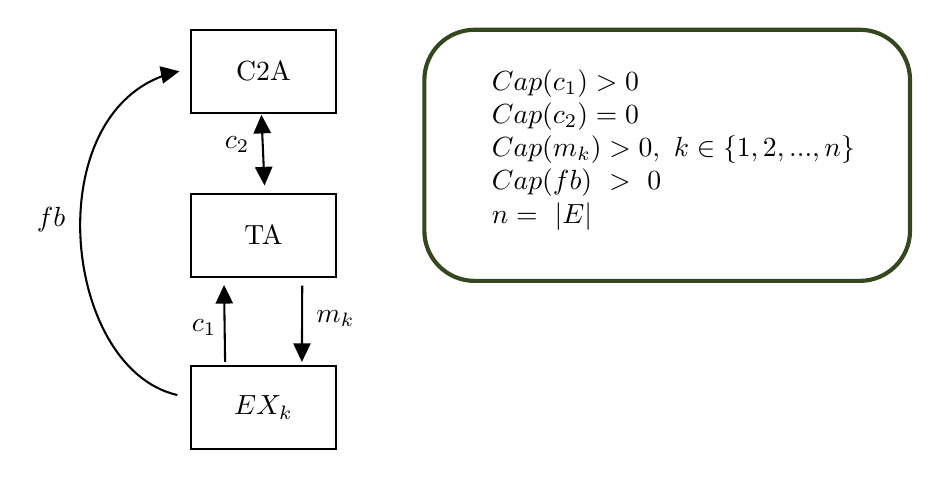
\begin{tikzpicture}[x=0.75pt,y=0.75pt,yscale=-1,xscale=1]
%uncomment if require: \path (0,229); %set diagram left start at 0, and has height of 229

%Shape: Rectangle [id:dp7793135649662085] 
\draw   (105,88) -- (175,88) -- (175,128) -- (105,128) -- cycle ;
%Shape: Rectangle [id:dp8388066725390221] 
\draw   (105,9) -- (175,9) -- (175,49) -- (105,49) -- cycle ;
%Shape: Rectangle [id:dp48691256180587716] 
\draw   (105,171) -- (175,171) -- (175,211) -- (105,211) -- cycle ;
%Straight Lines [id:da3337977868298102] 
\draw    (139.13,53) -- (140.37,81) ;
\draw [shift={(140.5,84)}, rotate = 267.47] [fill={rgb, 255:red, 0; green, 0; blue, 0 }  ][line width=0.08]  [draw opacity=0] (8.93,-4.29) -- (0,0) -- (8.93,4.29) -- cycle    ;
\draw [shift={(139,50)}, rotate = 87.47] [fill={rgb, 255:red, 0; green, 0; blue, 0 }  ][line width=0.08]  [draw opacity=0] (8.93,-4.29) -- (0,0) -- (8.93,4.29) -- cycle    ;
%Straight Lines [id:da7136052167478543] 
\draw    (158.67,132.33) -- (158.51,166) ;
\draw [shift={(158.5,169)}, rotate = 270.26] [fill={rgb, 255:red, 0; green, 0; blue, 0 }  ][line width=0.08]  [draw opacity=0] (8.93,-4.29) -- (0,0) -- (8.93,4.29) -- cycle    ;
%Straight Lines [id:da1199439366931846] 
\draw    (121.5,169) -- (121.04,135) ;
\draw [shift={(121,132)}, rotate = 449.23] [fill={rgb, 255:red, 0; green, 0; blue, 0 }  ][line width=0.08]  [draw opacity=0] (8.93,-4.29) -- (0,0) -- (8.93,4.29) -- cycle    ;
%Rounded Rect [id:dp3574279176331121] 
\draw  [color={rgb, 255:red, 53; green, 71; blue, 31 }  ,draw opacity=1 ][line width=1.5]  (217.5,33.2) .. controls (217.5,19.83) and (228.33,9) .. (241.7,9) -- (427.3,9) .. controls (440.67,9) and (451.5,19.83) .. (451.5,33.2) -- (451.5,105.8) .. controls (451.5,119.17) and (440.67,130) .. (427.3,130) -- (241.7,130) .. controls (228.33,130) and (217.5,119.17) .. (217.5,105.8) -- cycle ;
%Curve Lines [id:da7275055445236782] 
\draw    (98.5,185) .. controls (42.07,172.13) and (30.72,45.57) .. (97.45,29.45) ;
\draw [shift={(99.5,29)}, rotate = 528.53] [fill={rgb, 255:red, 0; green, 0; blue, 0 }  ][line width=0.08]  [draw opacity=0] (8.93,-4.29) -- (0,0) -- (8.93,4.29) -- cycle    ;

% Text Node
\draw (140,29) node   [align=left] {C2A};
% Text Node
\draw (140,108) node   [align=left] {TA};
% Text Node
\draw (140,191) node    {$EX_{k}$};
% Text Node
\draw (111.33,152.33) node    {$c_{1}$};
% Text Node
\draw (174.67,148) node    {$m_{k}$};
% Text Node
\draw (127.33,64.33) node    {$c_{2}$};
% Text Node
\draw (337.5,67) node    {$ \begin{array}{l}
Cap( c_{1})  >0\\
Cap( c_{2}) =0\\
Cap( m_{k})  >0,\ k\in \{1,2,...,n\}\\
Cap( fb) \  >\ 0\\
n=\ |E|\ 
\end{array}$};
% Text Node
\draw (37.67,100.67) node    {$fb$};


\end{tikzpicture}